\section{(Binäre) Bäume}


\begin{itemize}
    \item Der \textbf{Grad} eines Knotens ist die Anzahl seiner Nachfolger.
    \item Ein \textbf{innerer Knoten} ist ein Knoten mit Grad $\geq 1$.
    \item Ein Blatt ist ein Knoten mit Grad $0$.
    \item Der \textbf{Grad eines Baums} ist der maximale Grad eines Knotens im Baum (vgl.~\cite[102]{GD18c})

\item \end{itemize}


\noindent
Der \textbf{direkte linke} bzw. \textbf{direkte rechte Nachfolger} eines inneren Knotens ist sein linker bzw. rechter Nachfolger.\\

\noindent
Die \textbf{Tiefe} eines Knotens ist der Abstand des Knotens von der Wurzel, rekursiv definiert durch

\begin{equation}
    T(k) = \begin{cases}
            0 &\text{falls k Wurzel}\\
            1 + T(k') &\text{sonst}
    \end{cases}
\end{equation}

wobei $k'$ der direkte Vorgänger (``Elternknoten``) des Knotens $k$ ist.\\

\noindent
Die \textbf{Höhe} eines Baumes ist das Maximum der \textit{Tiefe} seiner Knoten\footnote{also der längste vorkommende Pfad,  von der Wurzel ausgehend}.\\

\noindent
Der Kurs definiert einen Baum als \textbf{vollständig}, wenn alle inneren Knoten zwei Söhne haben und alle Blätter die gleiche Tiefe\footnote{
    s. Skript (Teil 2) S. 101.
}.

\noindent
Die \textbf{maximale Höhe} eines Baumes ist $n - 1$ - diese wird in \textit{entarteten} Bäumen erreicht: Hier hat jeder Knoten maximal einen Nachfolger (vgl. Skript (Teil2) S.103).\\

\noindent
Die \textbf{minimale Höhe eines Baumes} ist $\lceil log_2(n + 1) \rceil - 1$: \textit{vollständige Bäume} besitzen minimale Höhe (vgl. Skript (Teil2) S.103).\\


\subsection{Preorder}
Wird ein Baum in \textbf{Preorder}-Reihenfolge traversiert, wird zunächst die Wurzel besucht, dann die Knoten des linken Teilbaums, dann die Knoten des rechten Teilbaums (\textit{KLR}).


\subsection*{Beispiel}
Sei der Baum wie in Abbildung~\ref{fig:bintree} gegeben\footnote{
die in diesem Abschnitt verwendeten Beispiele sind den Tutoraufgaben des SS2015, Lehrstuhls für Informatik 2, RWTH Aachen, entnommen (s. \url{https://moves.rwth-aachen.de/wp-content/uploads/SS15/dsal/Loesung2.pdf} - abgerufen 08.03.2024)
}.\\

\noindent
Die \textbf{Preorder}-Traversierung des Baumes ergibt  $3\ 4\ 2\ 7\ 1\ 5\ 9\ 1$.

\begin{figure}
    \begin{center}
        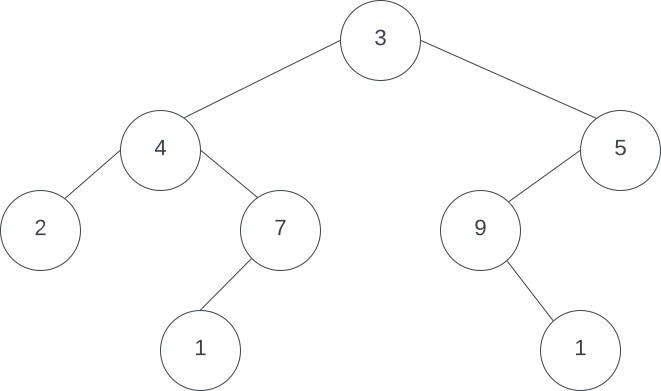
\includegraphics[scale=0.4]{chapters/Datenstrukturen und Algorithmen/img/bintree}
        \caption{Binärer Baum (Quelle: eigene)}
        \label{fig:bintree}
    \end{center}
\end{figure}

\subsection{Inorder}
Wird ein Baum in \textbf{Inorder}-Reihenfolge traversiert, werden zunächst die Knoten des linken Teilbaums besucht, dann die Wurzel, dann die Knoten des rechten Teilbaums (\textit{LKR}).

\subsection*{Beispiel}
Die \textbf{Inorder}-Traversierung des Baumes in Abbildung~\ref{fig:bintree} ergibt $2\ 4\ 1\ 7\ 3\ 9\ 1\ 5$.


\subsection{Postorder}
Wird ein Baum in \textbf{Postorder}-Reihenfolge traversiert, werden zunächst die Knoten des linken Teilbaums besucht, dann die Knoten des rechten Teilbaums, dann die Wurzel selber (\textit{LRK}) .

\subsection*{Beispiel}
Sei der Baum wie in Abbildung~\ref{fig:bintree} gegeben.\\

\noindent
Die \textbf{Postorder}-Traversierung des Baumes in Abbildung~\ref{fig:bintree} ergibt $2\ 1\ 7\ 4\ 1\ 9\ 5\ 3$.

\subsection{Rekonstruktion}
Ein binärer Baum lässt sich nur mit Hilfe der Inorder- \textit{und} der Pre- oder Postorder-Reihenfolge \textit{eindeutig} rekonstruieren.

\subsection*{Beispiele}
Sei folgende Inorder- und Preorder-Reihenfolge gegeben:\\

\noindent
Inorder: $5\ 8\ 4\ 7\ 3\ 1\ 6\ 9\ 2$\\
Preorder: $3\ 4\ 5\ 8\ 7\ 2\ 6\ 1\ 9$\\

\noindent
Der rekonstruierte Baum ist in Abbildung \ref{fig:inpre} dargestellt.\\

\begin{figure}
    \begin{center}
        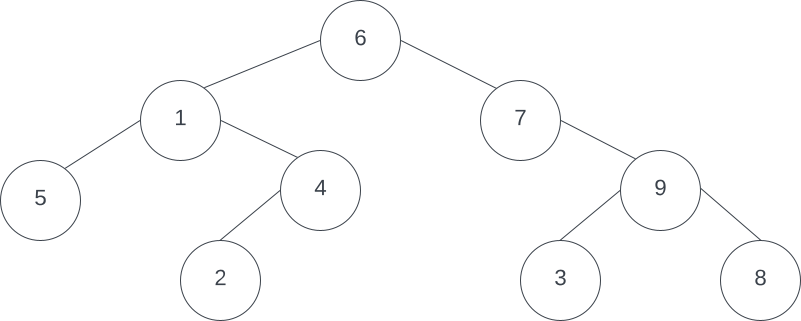
\includegraphics[scale=0.4]{chapters/Datenstrukturen und Algorithmen/img/inpost}
        \caption{Binärer Baum mit der Inorder-Reihenfolge $5\ 8\ 4\ 7\ 3\ 1\ 6\ 9\ 2$ sowie der Preorder-Reihenfolge $3\ 4\ 5\ 8\ 7\ 2\ 6\ 1\ 9$  (Quelle: eigene)}
        \label{fig:inpre}
    \end{center}
\end{figure}

\noindent
Sei folgende Inorder- und Postorder-Reihenfolge gegeben:\\

\noindent
Inorder: $5\ 1\ 2\ 4\ 6\ 7\ 3\ 9\ 8$\\
Postorder: $5\ 2\ 4\ 1\ 3\ 8\ 9\ 7\ 6$\\

\noindent
Der rekonstruierte Baum ist in Abbildung \ref{fig:inpost} dargestellt.


\begin{figure}
    \begin{center}
        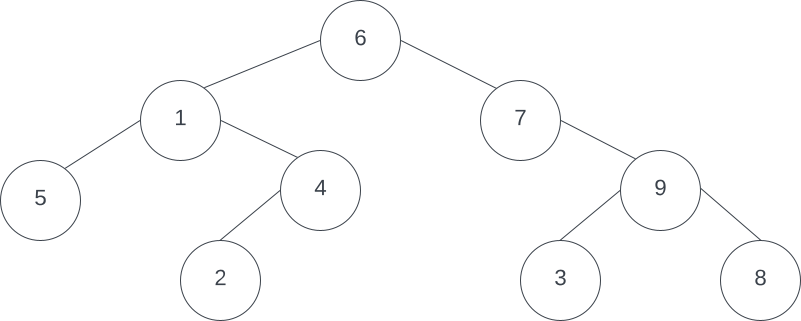
\includegraphics[scale=0.4]{chapters/Datenstrukturen und Algorithmen/img/inpost}
        \caption{Binärer Baum mit der Inorder-Reihenfolge $5\ 1\ 2\ 4\ 6\ 7\ 3\ 9\ 8$ sowie der Postorder-Reihenfolge $5\ 2\ 4\ 1\ 3\ 8\ 9\ 7\ 6$  (Quelle: eigene)}
        \label{fig:inpost}
    \end{center}
\end{figure}


\subsection{Einfügen / Suchen / Löschen in binären Suchbäumen}

Die Kosten für die Operationen \textit{Einfügen} / \textit{Suchen} / \textit{Löschen} belaufen sich auf $O(n)$, wobei $n$ die Anzahl der Knoten des Baumes ist.\\
Im worst-case ist ein Baum zu einer linearen Liste entartet\footnote{
    bspw. weil die einzufügenden Schlüssel schon sortiert vorliegen
}, so dass die komplette Liste durchlaufen werden muss, um ein Element in das Ende der Liste einzufügen bzw. zu überprüfen, ob das Element enthalten ist.\\

\noindent
Im Mittel wird für eine Einfügeoperation $O(log n)$ benötigt\footnote{
    vgl. \cite[136 ff.]{GD18d}
}.\\


\noindent
Der Aufwand für den Aufbau eines binären Suchbaumes Baumes mit $n$ bereits sortierten Elementen ist $O(n^2)$ (vgl.~\cite[235 f.]{GD18d}).


\subsection{Löschen}

In einem \textit{binären Suchbaum} gilt (rekursiv), dass der Schlüssel eines \textit{direkten linken Nachfolgers} \textbf{kleiner} als der Schlüssel seines \textit{direkten Vorgängers} ist.\\
Für den \textit{direkten rechten Nachfolger} gilt, dass sein Schlüssel \textbf{größer} als der Schlüssel seines direkten Vorgängers ist.\\

\noindent
Wenn in einem binären Suchbaum ein Knoten gelöscht wird, muss sein Ordnung wiederhergestellt werden.\\

\noindent
Dies erreicht man, indem man den gelöschten Knoten durch seinen \textbf{symmetrischen Nachfolger} bzw. \textbf{symmetrischen Vorgänger} ersetzt (vgl.~\cite[269, 272]{OW17e}).\\
Der \textbf{symmetrische Nachfolger} ist hierbei der Knoten im \textit{rechten} Teilbaum, der am weitesten \textit{links} steht ($\rightarrow$ kleinster Schlüssel im rechten Teilbaum).\\
Der \textbf{symmetrische Vorgänger} ist hingegen der Knoten im \textit{linken} Teilbaum,  der am weitesten \textit{rechts} steht($\rightarrow$ größter Schlüssel im linken Teilbaum).\\

\noindent
Generell wird beim Löschen so vorgegangen:

\begin{itemize}
    \item \textbf{Fall 1}: Der zu löschende Knoten ist ein Blatt
    \item [] In diesem Fall muss lediglich die Referenz auf das Blatt entfernt werden.
    \item \textbf{Fall2}: Der zu löschende Knoten hat nur einen direkten Nachfolger
    \item[] Die Referenz auf den zu löschenden Knoten wird auf den direkten Nachfolger gesetzt
    \item \textbf{Fall3}: Der zu löschende Knoten hat einen linken \textit{und} einen rechten Nachfolger
    \item[] Der zu löschende Knoten muss durch seinen symmetrischen Nachfolger oder Vorgänger ersetzt werden.
\end{itemize}\\


\noindent
Sei bspw. wie in Abbildung~\ref{fig:deltree} der binäre Suchbaum gegeben, dessen Knoten mit dem Schlüssel $5$ gelöscht werden soll.\\
Der symmetrische Nachfolger für diesen Knoten ist der Knoten mit dem Schlüssel $6$, der symmetrische Vorgänger ist der Knoten mit dem Schlüssel $4$ - beide kommen als Ersatz für den gelöschten Knoten in Frage.\\

\begin{figure}
    \begin{center}
        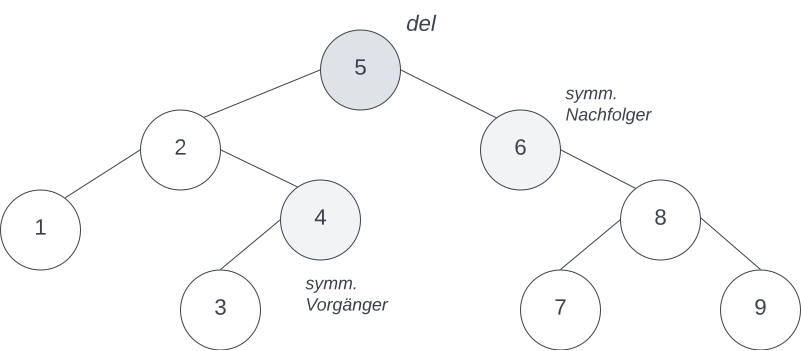
\includegraphics[scale=0.4]{chapters/Datenstrukturen und Algorithmen/img/deltree}
        \caption{Wenn der Knoten mit dem Schlüssel $5$ gelöscht wird, muss entweder der  Knoten mit dem Schlüssel $4$ an Stelle des gelöschten Knotens, oder der Knoten mit dem Schlüssel $6$, um die Ordnung in dem binären Suchbaum beizubehalten.(Quelle: eigene)}
        \label{fig:deltree}
    \end{center}
\end{figure}

\noindent
Es ist darauf zu achten, die Nachfolgerknoten / Vorgängerknoten beim Löschen korrekt umzuhängen:
\begin{itemize}
    \item \textbf{Fall 1}: Der symmetrische Vorgänger wird verwendet
    \item [] Da der symmetrische Vorgänger höchstens \textit{einen direkten linken Nachfolger} haben kann, wird dieser Knoten (in dem beispiel mit Schlüssel $3$) nun der neue \textit{direkte rechte Nachfolger} des direkten Vorgängers (Schlüssel $2$) des symmetrischen Vorgängers.
    Der neue direkte linke Nachfolger des Knotens mit dem Schlüssel $4$ wird der Knoten mit dem Schlüssel $2$.
    \item \textbf{Fall 2}: der symmetrische Nachfolger wird verwendet
    \item[] Da der symmetrische Nachfolger höchstens \textit{einen direkten rechten Nachfolger} haben kann, wird dieser Knoten nun der neue \textit{direkte linke Nachfolger} des direkten Vorgängers des symmetrischen Nachfolgers.
    In dem angegebenen Beispiel muss nichts weiter geschehen, da der direkte Vorgänger des symmetrischen Nachfolgers der zu löschende Schlüssel ist.
    Allerdings bekommt der Knoten mit dem Schlüssel $6$ nun einen neuen direkten linken Nachfolger, und zwar den Knoten mit dem Schlüssel $2$.
\end{itemize}\\


